\chapter{ランサムウェア対策}
\section{感染リスクの緩和}
現実世界の攻撃を戦術と使用技術の観点から分類したフレームワークであるMITRE ATT\&CK \cite{MITREATT12:online}によると,
ランサムウェアのデータ侵害は,攻撃の最終段階であるImpactステージの
Data Destruction,
Data Encrypted for Impact,
Data Manipulation
のいずれかに分類される.
つまり,ランサムウェアによるデータ侵害は初期アクセスや権限昇格などのステージを完了した後に発生するといえる.
したがって,本研究の提案手法のスコープ外であるが,
Impactより前のステージにおいてランサムウェアの感染リスクを緩和することもランサムウェア対策として重要であるため本節にて
概要を記載する.
\begin{figure}[t]
  \begin{center}
    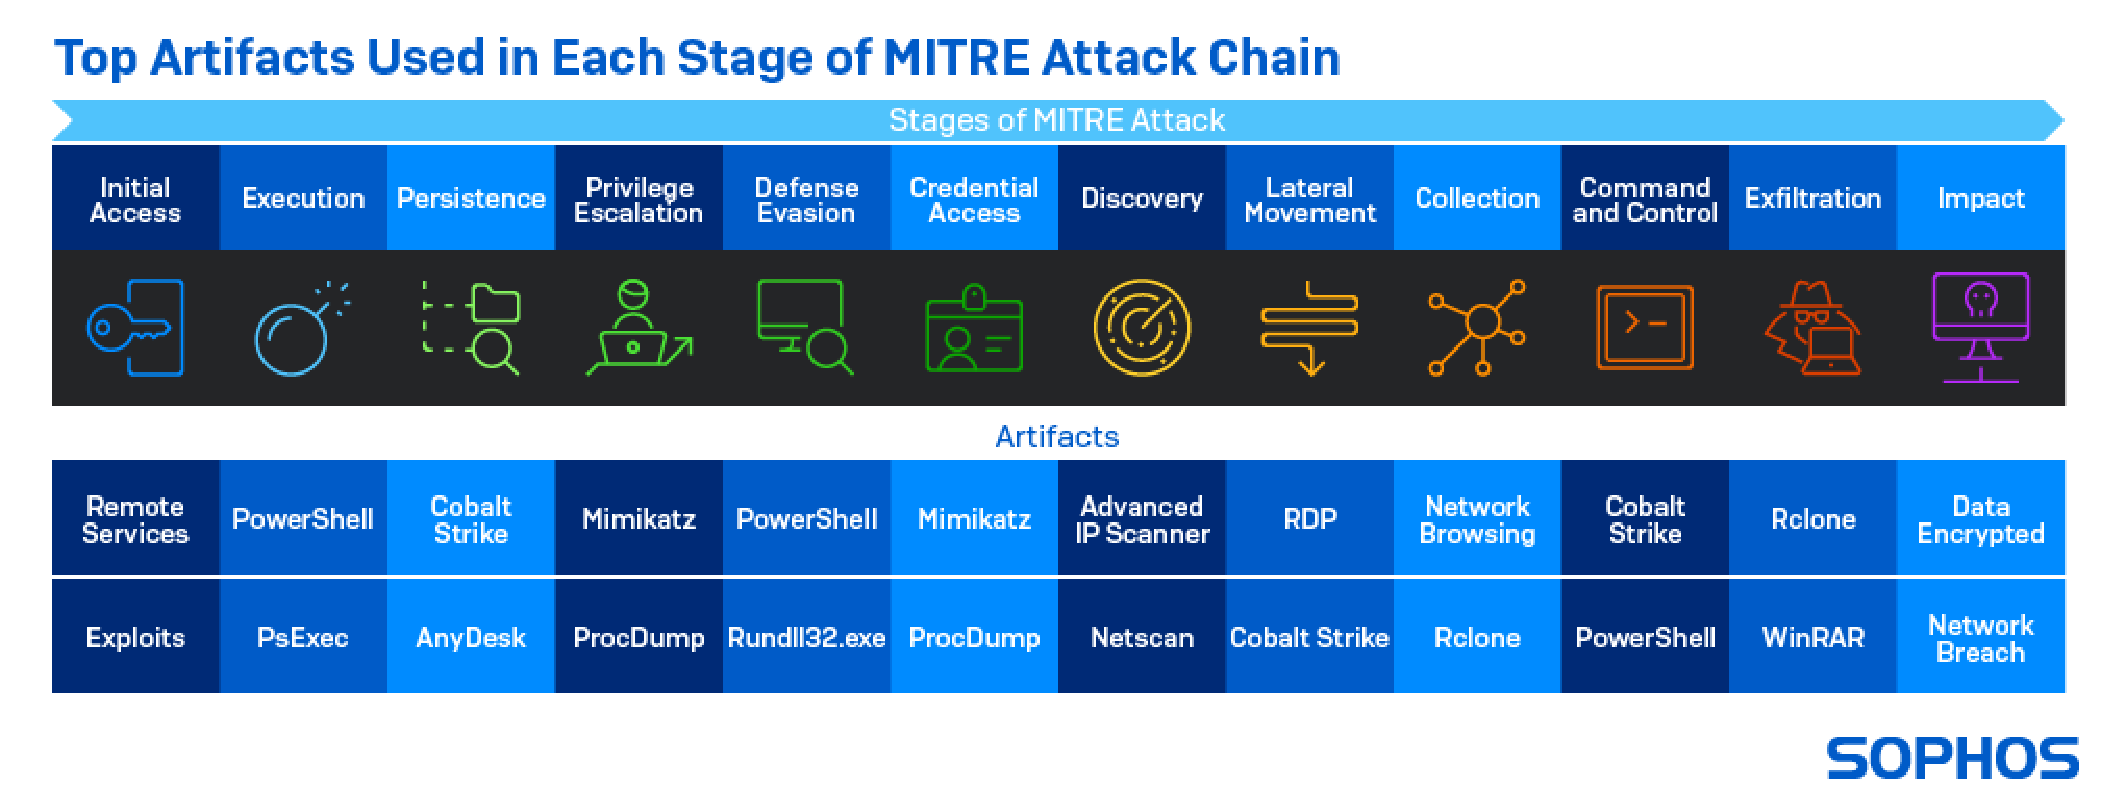
\includegraphics[width=\columnwidth]{doc/img/mitre-attack-chain.eps}
  \end{center}
  \caption{Overview of each stage in MITRE ATT\&CK framework.
    Some stages such as Reconnaissance are omitted for simplicity. \cite{mitre-explained}}
  \label{fig:mitre-attack-chain}
\end{figure}


